\documentclass[pra,twocolumn,showkeys,preprintnumbers, amsmath,amssymb, aps,A4paper]{revtex4-1}

\usepackage{amsmath}
\usepackage{graphicx}% Include figure files
\usepackage{dcolumn}% Align table columns on decimal point
\usepackage{array}
\usepackage{bm}% bold math
\usepackage{fancyvrb}


\newcommand{\ctu}{\cos(\theta_\uparrow)}


\begin{document}

%\preprint{SoftwareX/Elsevier}

\title{Restricted Boltzman Machine Variational parametrisation of Floquet operator}

\author{German A. Sinuco Leon}
\affiliation{School of Mathematics and Physical Sciences, University of Sussex, Falmer, BN1 9QH, United Kingdom.}


\date{\today}
\begin{abstract}

\end{abstract}

%\pacs{Valid PACS appear here}% PACS, the Physics and Astronomy
                             % Classification Scheme.
 
\keywords{ Multimode Floquet, Quantum dynamics, Dressed states, RBM, Machine Learning}
                              %display desired
\maketitle
\section{\label{sec:Introduction} Introduction}

%\begin{widetext}
\begin{figure}
\centering
%\includegraphics[width=0.8\linewidth]{GeneralDiscreteSystemSketch2.ps}
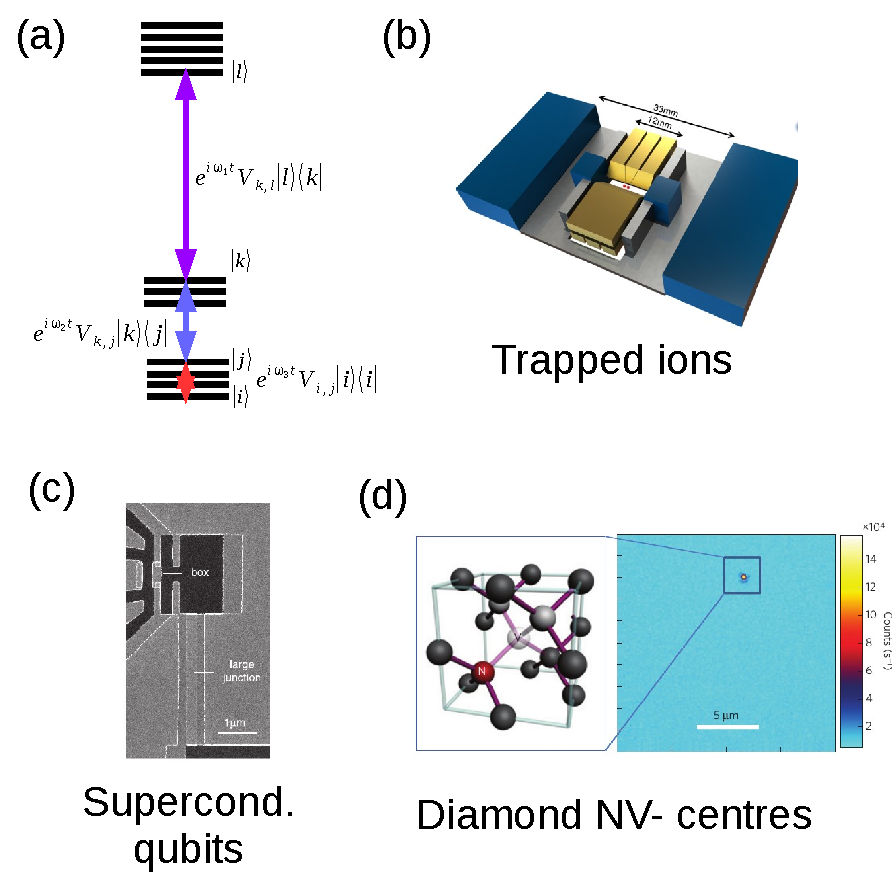
\includegraphics[width=0.8\linewidth]{GeneralDiscreteSystemSketch3.ps}
%\includegraphics[width=\linewidth]{figure1librarypaper.ps}
\caption{\label{fig:SystemSketch} (a) Schematic energy level structure of a generic quantum system. The basis of states consist of a discrete set of energy states, which define several bands according to the level energy spacing. Inter and intra band coupling is induced by electromagnetic radiation tuned at the corresponding frequencies, as indicated by the coupling terms. The wide variety of physical systems described by this model includes (b) trapped ions \cite{PhysRevLett.117.220501}, (c) superconducting qubits \cite{vion2002manipulating} and (d) diamond NV-centres \cite{balasubramanian2009ultralong}.}
\end{figure}
%\end{widetext}


\section{\label{sec:FloquetBloch} Floquet formalism}

The openMMF library is developed to calculate the time-evolution operator, $U(t',t), ~ t'>t$, of systems whose Hamiltonian has the form:
\begin{equation}
H = \sum_{i,j}^D E_{i,j} \left| i\right\rangle \left\langle j \right| + \sum_{i,j}^D \sum_{\ell=1}^N \sum_{n \in Z} V_{i,j}^{\ell,n} e^{i n \omega_\ell t} \left| i\right\rangle \left\langle j \right| + \textrm{h.c.}
\label{eq:Hamiltonian}
\end{equation}
where $D$ is the dimension of the Hilbert space, ${E_{i,j}}$ defines the static component of the Hamiltonian $H$, $V_{i,j}^{\ell,n}$ is the coupling between the states $i$ and $j$ oscillating at frequency $n \omega_{\ell}$ (i.e. the $n$-th harmonic of the $\ell$-th fundamental frequency $\omega_{\ell}$) and $N$ is the number of incommensurately frequencies.

To calculate the time-evolution operator we generalise the Rotating (or Resonant) Wave Approximation (RWA), taking into account the complex time dependence of eq. (\ref{eq:Hamiltonian}). For this, we rephrase the problem in terms of building a time-dependent unitary transformation, $U_F(t)$ to a new basis $\{\left| \bar{i} \right\rangle\}$, that leads to a \textit{time-independent} and diagonal Hamiltonian, $\bar{H}$. After applying the standard quantum-mechanical transformation rule to the Schr\"{o}dinger equation \cite{chu1985recent,PhysRevA.81.063626}, this condition becomes:
\begin{eqnarray}
 U_F^\dagger(t) \left[ H(t) - i \hbar \partial_t \right] U_F(t)  &=& \sum_{\bar{i}} \bar{E}_{\bar{i}} \left| \bar{i} \right\rangle \left\langle \bar{i} \right|
\label{eq:Hdressed}
\end{eqnarray}

Importantly, in the basis of states defined by this transformation the time evolution operator is diagonal and has the form:
\begin{equation}
\bar{U}(t',t) = \sum_{\bar{i}} e^{-i \bar{E}_{\bar{i}} (t'-t)} \left| \bar{i} \right\rangle \left\langle \bar{i} \right|
\label{eq:dressedtimeevolution}
\end{equation}
which let us to calculate the time evolution operator in the original basis $\left\{ \left| i\right\rangle\right\}$, just by inverting the transformation $U_F(t)$, according to \cite{PhysRevA.81.063626}:
\begin{equation}
U(t',t) = U_F(t') \bar{U}(t',t) U_F(t)
\label{eq:baretimeevolution}
\end{equation}

To formulate a fully defined computational problem, we express the micromotion operator $U_F(t)$ as the multifrequency Fourier series \cite{ho1983semiclassical}:
\begin{equation}
U_F(t) = \sum_{\vec{n}} U_{i,\bar{i}}^{\vec{n}} e^{-i\vec{\omega} \cdot \vec{n}t} \left| i \right\rangle \left\langle \bar{i} \right|
\label{eq:micromotionexpansion}
\end{equation}
where $\vec{\omega} = (\omega_1,\omega_2,\ldots,\omega_N)$ and $\vec{n}$ is a $N$-dimensional vector of integers. After plugging this expansion in eq. (\ref{eq:Hdressed}) and performing an integral over time, we obtain a fully defined eigenproblem for the eigenvalues $\bar{E}_{\bar{i}}$ and Fourier components of the unitary transformation $U_{i,\bar{E}}^{\vec{n}}$:
\begin{widetext}
\begin{equation}
\sum_j(E_{i,j} - \hbar \vec{n} \cdot \vec{\omega})U^{\vec{n}}_{j,\bar{i}} + \sum_{j} \sum_{\vec{m}} \left[ V^{\vec{m}}_{i,j} U^{\vec{n}+\vec{m}}_{j,\bar{i}} + V^{\vec{m}*}_{ji} U^{\vec{m}-\vec{n}}_{j,\bar{i}}\right] = \bar{E}_{\bar{i}}U^{\vec{n}}_{i,\bar{i}}
\label{eq:multimodeeigenproblem}
\end{equation}
\end{widetext}
where the couplings $V_{i,j}^{\ell,n}$ define $V_{i,j}^{\vec{n}}$ and the vector $\vec{n} = (0,\ldots , m, \ldots, 0)$ with the value $m$ located at the $\ell-$th position. To obtain a finite matrix representation of this problem we truncate the sum over the number of modes of the Fourier expansion eq. (\ref{eq:micromotionexpansion}). Below, in Appendix A, we show an specific example of the shape of the matrix for a bichromatic driven problem. 

This formulation to calculate the time-evolution operator is equivalent to the multimode Floquet representation of the Hamiltonian that introduces the extended Hilbert space $\left| E_i,\vec{n} \right\rangle$  \cite{shirley1965solution,ho1983semiclassical,verdeny2016quasi}. However, the semiclassical description presented here makes emphasis in the experimentally accessible states, which usually are used to express the static part of the Hamiltonian eq.  (\ref{eq:Hamiltonian}). 


\section{RBM parametrisation of the micromotion operator}

\begin{figure}[!htb]
\centering
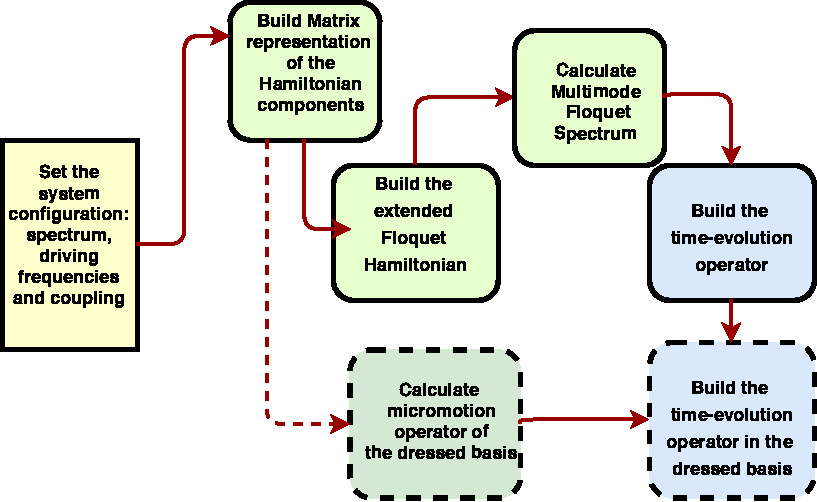
\includegraphics[width=0.8\linewidth]{MultimodeFloquetFigure1.ps}
\caption{\label{fig:FlowChart} Typical sequence of function calls to calculate the time-evolution operator of a quantum system with the openMMF library.}
\end{figure}

\section{Dressed spectrum}
\subsection{Eigenenergies}
\subsection{eigenstates}

\section{\label{sec:sequence} Outlook}
Considering that a wide diversity of physical systems are described by the Hamiltonian in eq. (\ref{eq:Hamiltonian}), the openMMF library constitutes a general purpose tool for studying quantum dynamics of driven systems. The library is open-source and provides a ready-to-use interface, which can be exploited by users with a broad range of expertise ranging from graduate students to established scientific researchers. An important feature of the library is the set of functions that allow the user to evaluate the time-evolution in a dressed basis, which is of current interest across different fields. To illustrate the degree of generality of the library, and therefore its potential impact, here we mention three specific research areas where the openMMF library can find direct application.

\bigskip
\noindent
\textit{Coherent control of quantum systems}

Precise control over the state of a quantum system is key for quantum technologies. An important operational step in such applications is the precise creation of quantum superposition, which is generally achieved by interleaving periods of free and driven evolution described by a Hamiltonian of the form eq. \ref{eq:Hamiltonian} \cite{macquarrie2015continuous}.  Decoherence induced by the interaction of the system with the environment is a major obstacle to achieve the levels of control required for the realisation of practical applications. However, superposition of dresses states can be more robust to environmental noise than bare states.  This mechanism to reduce the sensitivity of a quantum system to noise is known as Continuous Dynamical Decoupling and, to be implemented, it requires an experimental sequence that follows the  path  schematically shown in figure \ref{fig:DressedBasis}. This technique has  improved the coherence of atomic clocks \cite{sarkany2014controlling,PhysRevA.97.013407} and qubit gates \cite{randall2015efficient, PhysRevLett.113.237601}, as well as for improved sensitivity, spatial resolution of magnetometers operating in the challenging regime of low-frequencies \cite{hirose2012continuous,baumgart2016ultrasensitive,yan2013rotating}. 

%Concatenated continuous decoupling: NJP 14, 113023 (2012), PRA 97 (2018) 013407

\bigskip
\noindent
\textit{Time-domain quantum simulations}

%\begin{figure}[!htb]
%\centering
%\includegraphics[width=0.5\textwidth]{figuretimedomainlattice.ps}
%\caption{\label{fig:timedomainlattice}Equivalent representation of a multimode driven quantum system (here bichromatic). (a) Time-dependent couplings in the Hilbert space of the system. (b) Equivalent lattice representation. Colour arrows represent AC couplings. }
%\end{figure}

The frequency-domain representation of the Hamiltonian eq. (\ref{eq:Hamiltonian}) with $N$ mutually irrational frequencies is given by eq. (\ref{eq:multimodeeigenproblem}). This representation can be interpreted as the  Hamiltonian of an $N$-dimensional lattice with sites label by the index $\vec{n}$,  a DC force equal to $\vec{\omega}$ and couplings between sites controlled by the driving modes. The typical signatures of dynamics of the simulated lattice (e.g. band structure, conductivity, edge-states, etc.) arise in the time-evolution of the system, which is directly accessible with the openMMF library. Topologically non-trivial states \cite{ma2018experimental,martin2017topological} and Anderson localisation in quasi-crystals \cite{delande2017three} are two phenomena accessible with this scheme for quantum simulations, which could be realised with a significantly simple experimental setups.


\bigskip
\noindent
\textit{Out-of-equilibrium phases of driven interacting systems}

The behaviour of driven systems can be qualitatively very different from their static counterparts. Different driving schemes has been recently used to engineer effective Hamiltonian displaying out-of-equilibrium phases that are impossible to realise with static systems \cite{PhysRevB.82.235114}. In the single particle case, the dynamics in the limits of high frequency or strong and resonant driving are relatively well understood \cite{PhysRevB.91.245135}, and novel phases of matter in such regimes has been proposed and realised in recent years \cite{desbuquois2017controlling,nakajima2016topological}. However, there are a number of fundamental questions  still to be addressed in the context of many-body driven systems, which emerge from the interplay between interactions, driving and symmetries/disorder \cite{delande2017three, PhysRevLett.116.250401}. The openMMF library provides a tool for exact diagonalisation calculations to investigate such phenomena. Though current computational limitations allows only to investigate systems with relatively small Hilbert space dimension, such studies provide solid understanding of the non-equilibrium dynamics of driven systems \cite{PhysRevLett.119.123601,PhysRevLett.121.050602,PhysRevLett.121.076802} and the library provides a platform of simple usability.

In this paper we introduce the openMMF library as a tool to calculate the time-evolution operator of quantum systems with discrete spectrum driven by harmonic couplings. The library implements the multimode Floquet expansion of a time-dependent Hamiltonian and provides several functionality relevant for its analysis. In particular, the library allows the user to evaluate the micromotion operator associated to arbitrary drivings built as superposition of harmonic terms. In passing, this procedure generalises the notion of dressed states to such situations. 

The general formulation implemented in the library enables its use for applications where determining the time-evolution operator is relevant, such as designing optimal control sequences, tailoring the response of quantum systems and studying non-equilbity quantum dynamics. The code is written in Fortran 90 and we provide  wrappers for C++, making it widely accessible and easy usage. 



\bibliography{LibraryBib}


\section*{Acknowledgements}
We acknowledge fruitful comments and input from Dr. Juan Sebastian Totero Gongora. This work has been supported by the School of Mathematics and Physics of the University of Sussex.

\section*{Appendix A: Typical example of the matrix representation of the multimode Hamiltonian}

A typical shape of the matrix representation of the RHS of eq. (\ref{eq:multimodeeigenproblem}). Here we consider a static system $H_0$ driven by the three frequencies: $\omega_1,2\omega_1,\omega_2$. The integer array describing this set of frequencies must be $(0,2,1)$. For the two fundamental frequencies, the number of Fourier modes in the decomposition of the micromotion operator is chosen to be $N_F=3$. With this, the driving of  $\omega_1$ and its first harmonic leads to the matrix:

\begin{widetext}
\[
\mathcal{H}_1 = \begin{pmatrix}
 H_0 + 3 \hbar \omega_1 & V^{1,1} & V^{1,2} & 0 & 0 & 0 &0 \\
  V^{1,1\dagger} & H_0 + 2 \hbar  \omega_1 & V^{1,1} & V^{1,2} & 0 & 0 & 0 \\
 V^{1,2 \dagger} &  V^{1,1\dagger} & H_0 + \hbar \omega_1 & V^{1,1} & V^{1,2} & 0 & 0 \\
 0 &V^{1,2 \dagger} &  V^{1,1 \dagger} & H_0  & V^{1,1}  & V^{1,2} & 0  \\
 0 & 0 &V^{1,2 \dagger} &  V^{1,1 \dagger} & H_0 - \hbar \omega_1 & V^{1,1} & V^{1,2}   \\
 0 & 0 & 0 &V^{1,2 \dagger} &  V^{1,1 \dagger} & H_0 - 2 \hbar \omega_1 & V^{1,1} \\
 0 & 0 & 0 & 0 &V^{1,2 \dagger} &  V^{1,1 \dagger} & H_0 - 3 \hbar \omega_1 
\end{pmatrix}
\]
\noindent
and the full matrix results in:
\[
\mathcal{H} = \begin{pmatrix}
 \mathcal{H}_1 + 3 \hbar \omega_2 & \mathcal{V}^{2,1} & 0 & 0 & 0 & 0 &0 \\
  \mathcal{V}^{2,1\dagger} & \mathcal{H}_1 + 2 \hbar  \omega_2 & \mathcal{V}^{2,1} & 0 & 0 & 0 & 0 \\
 0 &  \mathcal{V}^{2,1\dagger} & \mathcal{H}_1 + \hbar \omega_2 & \mathcal{V}^{2,1} & 0 & 0 & 0 \\
 0 & 0 &  \mathcal{V}^{2,1 \dagger} & \mathcal{H}_1  & \mathcal{V}^{2,1}  &0 & 0  \\
 0 & 0 & 0 &  \mathcal{V}^{2,1 \dagger} & \mathcal{H}_1 - \hbar \omega_2 & \mathcal{V}^{2,1} & 0   \\
 0 & 0 & 0 &0 &  \mathcal{V}^{2,1 \dagger} & \mathcal{H}_1 - 2 \hbar \omega_2 & \mathcal{V}^{2,1} \\
 0 & 0 & 0 & 0 & 0 &  \mathcal{V}^{2,1 \dagger} & \mathcal{H}_1 - 3 \hbar \omega_2
\end{pmatrix}
\]
with
\[
\mathcal{V}^{2,1} = \begin{pmatrix}
  V^{2,1} & 0 & 0 & 0 & 0 & 0 &0 \\
  0&V^{2,1} & 0 & 0 & 0 & 0 & 0  \\
  0&0&V^{2,1} & 0 & 0 & 0 & 0  \\
  0&0&0&V^{2,1} & 0 & 0 & 0 \\
  0&0&0&0&V^{2,1} & 0 & 0  \\
  0&0&0&0&0&V^{2,1} & 0 \\
  0&0&0&0&0&0&V^{2,1}  
\end{pmatrix}
\]
\end{widetext}

\section*{C++ wrapper}
The library includes wrappers to use with C++. The interfaces to the Fortran subroutines  share the name of the aimed function with the appended particle \verb _C_ .  The full set of wrappers are declared in the file \verb MultimodeFloquet.h  , which must be included in the C++ source code. As an example we present  the C++  codes required to evaluate the time-evolution of a driven qubit. The library distribution includes Fortran and C++ examples.

\begin{widetext}
\begin{verbatim}

#include <iostream>
#include <complex>
#include <stdio.h>
#include <math.h>
#include <string.h>

using namespace std;
typedef std::complex<double> dcmplx;

#include "MultimodeFloquet.h"

extern "C" int h_floquet_size;

int main(){

  atom_c id;
  int info,N_;
  int jtotal;
  char name[]     = "qubit";
  char manifold[] = "U";

  int r,m,l;
  int d_bare,total_frequencies;

  double t1,t2;

  info   = 0;
  jtotal = 2;
  floquetinit_c(&id,name,&info);

  d_bare = id.d_bare;

  dcmplx * U_AUX = new dcmplx [d_bare*d_bare];

  int nm = 2;
  int * modes_num = new int [nm];

  modes_num[0] = 1;
  modes_num[1] = 1;
  
  total_frequencies = 0;
  for(r=0;r<nm;r++){
    total_frequencies += modes_num[r];
  }
  
  mode_c * fields = new mode_c [total_frequencies];
  

  // --- SET DRIVING PARAMETERS   
  fields[0].x    = 0.0;
  fields[0].y    = 0.0;
  fields[0].z    = 2.0;
  fields[0].phi_x = 0.0;
  fields[0].phi_y = 0.0;
  fields[0].phi_z = 0.0;
  fields[0].omega = 0.0;
  fields[0].N_Floquet = 0;

  fields[1].x     = 4.0;
  fields[1].y     = 0.0;
  fields[1].z     = 0.0;
  fields[1].phi_x = 0.0;
  fields[1].phi_y = 0.0;
  fields[1].phi_z = 0.0;
  fields[1].omega = 2.0;
  fields[1].N_Floquet = 3;

  // --- SET THE HAMILTONIAN COMPONENTS
  sethamiltoniancomponents_c_
               (&id,&nm,&total_frequencies,modes_num,fields,&info);
    
  // --- BUILD THE MULTIMODE FLOQUET MATRIX AND  FIND ITS SPECTRUM     
  multimodefloquetmatrix_c_
   (&id,&nm,&total_frequencies,modes_num,fields,&info);

  double * e_floquet = new double [h_floquet_size];
  dcmplx * U_F =  new dcmplx [h_floquet_size*h_floquet_size];
    
  lapack_fulleigenvalues_c_
   (U_F,&h_floquet_size,e_floquet,&info);
// the diagonalization is done with the internal (Fortran)
// Hamiltonian (H_FLOQUET) and the calculated
// U_F is the transformation that diagonalise this Hamiltonian
// On the Fortran side, H_FLOQUET is deallocated after
// diagonalization. 

   //--- EVALUATE TIME-EVOLUTION OPERATOR IN THE BARE BASIS

   N_ = 256;
   t1= 0.0;
   for(r=1;r<N_;r++){      
     t2 = r*100.0/N_;
     multimodetimeevolutionoperator_c_
       (&h_floquet_size,&nm,modes_num,U_F,e_floquet,&d_bare,fields,&t1,&t2,U_AUX,&info);
     for(l=0;l<d_bare*d_bare;l++) p_avg[l] = pow(abs(U_AUX[l]),2);
     write_matrix_c_(p_avg,&d_bare);           
   }
    delete(e_floquet);    
    delete(U_F);
  }
  
  return 0;
}

\end{verbatim}
\end{widetext}

\end{document}
